\documentclass{article}
\usepackage[english]{babel}
\usepackage[utf8]{inputenc}
\usepackage[T1]{fontenc}
\usepackage{amsmath,amssymb,amsfonts}

\usepackage{xspace}
\usepackage{graphicx}
\usepackage{color}
\newcommand{\system}{MADden\xspace}

\title{MADden : In-Database Text Analytics}
\author{Morgan Bauer 9890-4838 \\
  Christan Grant 8143-3970 \\
  Joir-dan Gumbs 6148-9357}
\date{December 13, 2011}
\begin{document}
\maketitle

\begin{figure}
  \begin{center}
    
\includegraphics[width=104mm]{logo.png}
    \caption{logo for overarching project}
    \label{fig:logo}
  \end{center}
\end{figure}

\begin{enumerate}
\item Names of the group members and UFIDs

  % not sure if it's best to put this into the public with our uf-id on it ~mhb

  Morgan Bauer

  Christan Grant

  Joir-dan Gumbs

\item Title of the project and abstract

  MADden : In-Database Text Analytics

  ABSTRACT



\item Final report should include the following topics:

  \section{Introduction (1 page)}

  MADlib, MAD, Magnetic Agile Deep.
  Madlibs, fill in the blank games, that usually have amusing and unforeseen outcomes.
  MADden, our initial problem domain deals with football,
  and John Madden is a famous former player, coach, and commentator,
  also known for the long-running series of video games that bear his name.

  \begin{enumerate}
  \item The problem statement and a summary of the main contributions and results of the project.

    Problem is he large amounts of structured and unstructured data that is available, and how to intermix the two.
    We use statistical text analysis techniques to extract structured information from unstructured data,
    and pass this on to later stages for further processing.

    We provide the ability to run queries over heterogeneous data such as structured statistical facts and unstructured natural language.

    Scraping dirty data and turning it into clean information, and then presenting the information in an easy to digest form.


    Goal of tinkering with sports data for gaining insight of team/player performance and fan sentiment.'

    We do however hope to be generic, and liberal in the data we take in, so that the same techniques can be applied to multiple domains.

    There is a web interface that provides preassembled queries that can be filled in like the madlibs game.
    It serves as a proving ground for various queries we test and run.

  \item What is the responsibility of each member of the group?



    Morgan did consulting work among the various group members, and between groups.
    Official NFL team blogs. NFL stats from cbssports.com.
  \end{enumerate}

  \section{Background (1 page)}
  \subsection{Domain}

  Our initial domain is the National Football League (NFL).
  This would be useful for a sports journalist to do computational/digital journalism.
  Covering all 32 teams with more than 1700 players is made manageable.
  A sports journalist would need a system
  that can analyze both the
  structured statistics (e.g., scores, biographic data) of teams and players and the
  unstructured tweets, blogs, and news about the games.



  \subsection{Background Information}
  \begin{enumerate}
  \item Background information (basic concepts, algorithms, etc.)



  \item Statistical Text Analysis Tools - list them and give a short description

    Text analysis uses the state-of-the-art statistical machine learning (SML) methods to extract structured information,
    such as entities, relations, sentiments, topics, from text.

    The result of the text analysis can be joined with other
    structured data sources to perform analysis. For example, the sports
    journalist may want to join the sentiment result from tweets and the
    scores of the Arizona Cardinals\footnote{http://www.azcardinals.com}
    (NFL Team) to see their correlations.


  \item Part of Speech (POS) Tagging is the basis of further querying.


  \item Sentiment

    Sentiment analysis extracts the polarity of subjective opinions from documents.
    These subjective feelings are important for assessing the popularity of subjects,
    and can be used to establish the collective feelings of the public on a subject.

  \item Information Extraction (IE) is the concept of identifying objects of interest,
    using relations present in the data.
    This varies from simple relations between subjects,
    to recognizing specific entities within text.


  \item Entity Resolution (ER) is the processing of recognizing and disambiguating different subjects in a document.
    That is, recognizing that people are present,
    or mentioned, and knowing who they are.

    Where as IE was concerned about the existence of various objects,
    and identifying their existence,
    ER is concerned with taking these entities and knowing whether they are the same or different.


  \item Conditional Random Fields (CRF) are a type of graphical model.
    A CRF is a supervised learning algorithm, requiring labeled training examples.
    In our case we are using CRFs to label sequences of natural language text.
    The quality and breadth of this set determines how well the trained CRF performs.
    They can be used for different things depending on their training set.
    We intended to use CRFs for POS tagging, IE, and ER.

    We have an implementation of the CRF evaluation, that uses a provided model, and labels sequences in the database.
    This is done using the forward-backward algorithm and the Viterbi algorithm, which are both instances of dynamic programing.

    (viterbi, forward-backward, linear vs skip-chain) evaluation over pre-trained model done in database.

  \end{enumerate}
  \subsection{Related work}

  related work

  MADlib, directly

  NLTK, POS Tagging, among other things.

  Twitter sentiment, for twitter sentiment. maybe reference whatever is being worked on with Wilson involving this.

  IIT for CRF training.

  Wang et al. for idea of doing CRF in database

  \subsection{Our Uniquness}
  How is this project different from related work

  Integration of analysis queries into the database.
  Ability to build ad hoc queries, as if they fit.

  Using {\system} we are able to perform a declarative query over the data set to return related documents.
  This is a ``what we want, not how to get it'' style query.

  \section{System Description (4 pages)}
  \subsection{System Architecture}
  What is the final system architecture?

  {\system} is a four layered system, as can be seen in Figure \ref{fig:arch}.
  The user interface is where both naive and advanced users can construct queries over text, structured data, and models.
  From the user interface,
  queries are then passed to the DBMS,
  where MADLib and {\system} libraries sit on top of the query processor to add statistical and text processing functionality.
  % These queries are processed using PostgreSQL/Greenplum's Parallel DB architecture to further optimize on replicated storage.


  \subsection{System Components}
  What are the system components and statistical methods developed?

  PostgreSQL, with MADlib overtop.
  Hope to scale up and use greenplum parallel DB.

  There is a new feature for MADlib that implements CRF evaluation, but not training, in the database.
  CRF specifically -

  The full text search capabilities of PostgreSQL are leveraged,
  as is the technique of inverted indexing.


  Statistical Text Analysis Tools - in depth description of how they were performed.
  \begin{enumerate}
  \item information extraction

    Verbatim from previous paper.

    Once we have the text documents, we would like to then be able to identify
    objects of interest. Information Extraction methods become increasingly
    important as the size of our corpus gets large. Many methods exist for in-database data
    extraction, but we are currently focused on building upon existing work in
    utilizing Conditional Random Fields (CRFs) for query-time extraction of
    entities.

    This would be applied to the unstructured twitter data,
    and the semi-structured play-by-play data,
    possibly with a specialized CRF for each of them.
    As well, this would be applied for Named Entity Recognition purposes to general text, for identifying players and teams.

  \item entity resolution

    What it is -
    This links various forms and representations of the same background object,
    so that a query for one of them returns the results for all of them.

    Why is it necessary -
    This is necessary for two reasons,
    the informality of speaking in documents like blog posts and twitter tweets,
    which leads to misspellings and slang
    and the more  general case of people or companies having many names to refer to them.

    Example of informality, slang \& misspelling. tmrw, tomorrow. NY Jest, NY Jets.

    Example of multiple names for a person.
    Nickname for Larry Fitzgerald, Sticky Fingers.
    Company Name and Acronym and Nickname, International Business Machines, IBM, Big Blue.
    New York City, Big Apple.

    Example of multiple things with one name.
    Arizona Cardinals, cardinals as a bird.
    Miami Dolphins, dolphins as a fish, dolphins as a mammal


    This is implemented through q-grams for misspellings and alternate spellings,
    and an alias table for multiple names of an entity.
    q-grams is the automatic approach that does fuzzy string matching,
    with a threshold value that can be varied.
    The alias table being hand constructed.


  \item TODO: Q-grams - description and example here

    \begin{tabular}{cc}
      VOTKA & VODKA \\ \hline
      {\color{green}\#\#V} & {\color{green}\#\#V} \\
      {\color{green}\#VO} & {\color{green}\#VO} \\
      {\color{red}VOT} &  {\color{red}VOD} \\
      {\color{red} OTK} &{\color{red} ODK} \\
      {\color{red} TKA} &{\color{red} DKA} \\
      {\color{green}KA\$} & {\color{green}KA\$} \\
      {\color{green}A\$\$} &  {\color{green}A\$\$} \\
    \end{tabular}

    Resolving the multiple things with one name, was not tackled. (as far as I can tell mhb)

    We also have a basic hookup to NLTK, to do basic named entity recognition.

  \item sentiment analysis

    Sentiment analysis extracts the polarity of subjective opinions from documents.
    The current implementation returns sentiment as a trinary option of positive, neutral, or negative.
    We would like to have more gradations in the extremeness of the opinion,
    as well as analysis of an opinion pertaining to a certain subject, or entity, that has been extracted.

    Currently this is handled as a UDF which makes an out of database call across the network.
    It also does this on a document by document basis,
    when the submission API supports batches of documents.
    Priority should be given to establish batch submissions,
    followed by writing the UDF as a local function,
    and possibly an in-database function.

    JSON API.


  \item part of speech tagging

    Part of Speech Tagging (POS tagging) labels each token of a sequence with a tag based on the grammar of a natural language.
    These tags are parts of speech, based on context and word definitions.
    The generators for these tags can come from both supervised and unsupervised sources.
    Statistical methods are used to generate taggers specific to a corpus, and thus a particular subject.
    These parts of speech are useful in other stages, such as entity resolution and information extraction (ER \& IR).

    Using CRF -
    Initially trained on email headers.
    This data was not generic enough to be useful.
    The individual documents were to small and not of a form similar enough to ensure correct tags.

    The next CRF was trained using (email contents)? .
    While it had a higher accuracy, the training corpus was probably too small (only 100 or 200 documents right?).
    The tagging accuracy was higher than the previous CRFs

    We need to train a CRF specific to our domain,
    and would like to train a CRF specific to each type of text,
    such as a twitter CRF, a blog CRF, etc.

    Using NLTK -
    Our current system does not utilize the CRF style model.
    Instead, as a UDF, we make a call to the Python Natural Language Toolkit (NLTK).
    (what kind of tagger is this? Brill? Naive Bayes? I don't know where the sourcecode is. ~mhb)
    This returns the tagged data, which can be used in PostgreSQL for later stages of analysis.


  \end{enumerate}





  \begin{figure}
    \begin{center}
      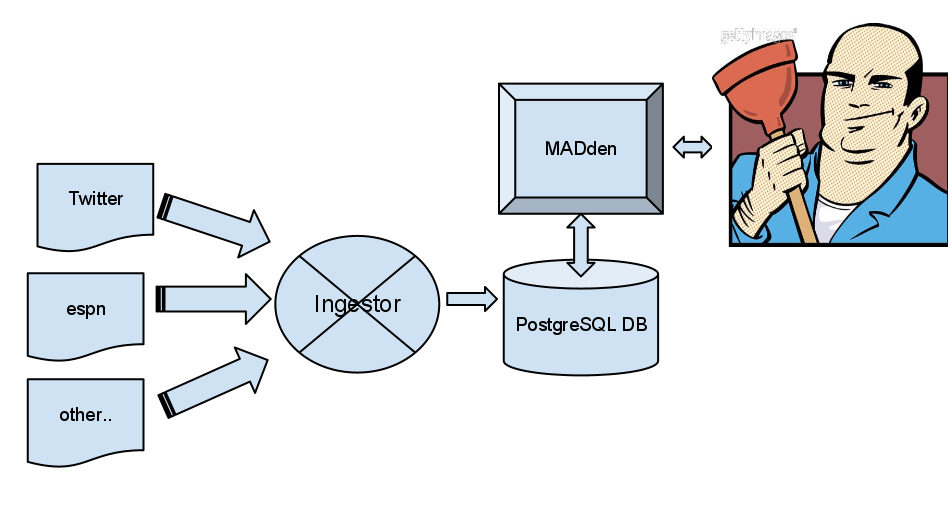
\includegraphics[width=104mm]{architecture-1.png}
      \caption{System Architecture}
      \label{fig:architecture}
    \end{center}
  \end{figure}

  \begin{figure}
    \begin{center}
      \includegraphics[scale=0.4]{arch.png}
      \caption{{\system} architecture}
      \label{fig:arch}
    \end{center}
  \end{figure}


  \begin{figure}
    \begin{center}
      \includegraphics[scale=0.4]{altarchitecture.png}
      \caption{{\system} architecture}
      \label{fig:altarch}
    \end{center}
  \end{figure}


  \begin{figure}
    \begin{center}
      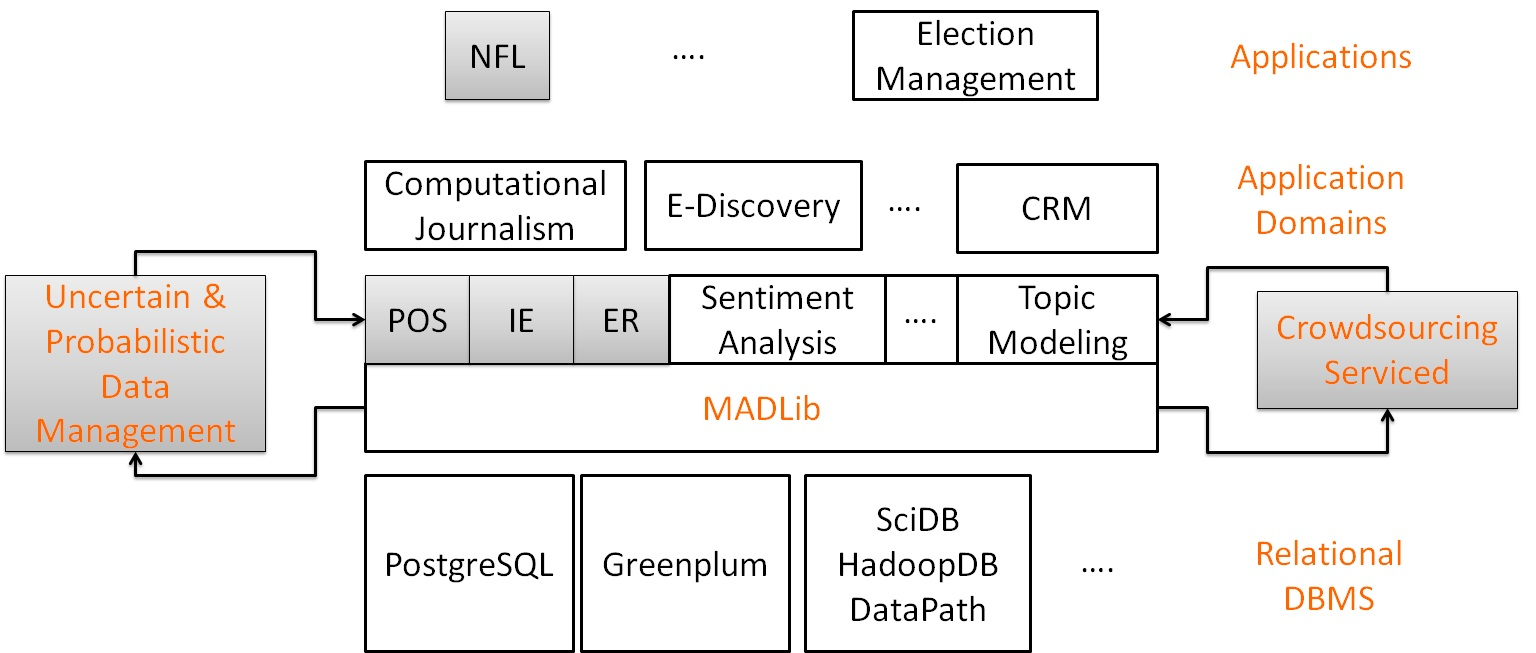
\includegraphics[scale=0.4]{altarchitecture2.png}
      \caption{{\system} architecture 2}
      \label{fig:altarch2}
    \end{center}
  \end{figure}



  \subsection{Data Products}
  What are the final data products?

  We don't have particular products, so much as abilities to deliver varying products, and adapt to the data as it changes.

  Ad hoc queries

  From first proposal:
  \begin{enumerate}
  \item[1] Correlations between game actions, such as:
    \begin{enumerate}
    \item[A] Outcome of coin toss for home/away team
    \item[B] Probability of making field goal based on
      stadium (by distance of attempt)
    \item[C] Fan sentiment with game outcome.
    \end{enumerate}
  \item[2] Summary of team performance
  \item[3] Tweet density for every game
  \item[4] ... and other things yet to be discovered
  \end{enumerate}

  \begin{figure}
    \begin{center}
      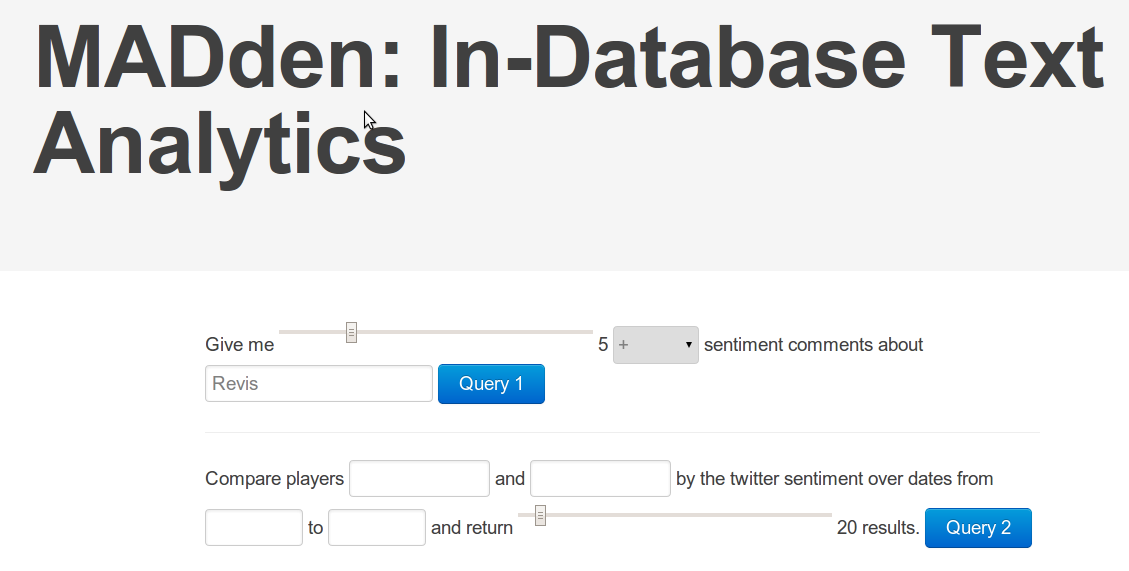
\includegraphics[scale=0.3]{web-ui.png}
      \caption{{\system} Web UI}
      \label{fig:web-ui}
    \end{center}
  \end{figure}

  \section{Experiments (2 pages)}
  \begin{enumerate}
  \item What datasets have been used? What’s the measure of success?

    Datasets
    % my description of document size is vague ~mhb

    Twitter -- unstructured, microblogs, very small document size (140 characters). This was gathered using the twitter trickle. With domain related terms, like NFL, Tim Tebow, Jets.
    Approximately 9GB of tweets, yielding a 7GB inverted index.

    Blogs -- english language, small-medium document size, 10-100 sentences.
    30k+ from official NFL teams, going back several years.
    60k+ from ESPN as commentary going back several years.

    play-by-plays -- semi-structured, repeated patterns with specific meaning.


    Measure of success?

    Do we get sane output? Yes.

  \item What are the main experimental results? Effectiveness/performance?

    Throughput for sentiment analysis is dominated by making a remote call.

    Throughput for POS tagging is dominated by making a python call (interpreted).

  \end{enumerate}

  \section{Conclusion (1 page)}
  \begin{enumerate}\item What you have learnt through this project?

    Morgan - learned how to parse html. write and use a webcrawler. CRF stuff. Database stuff.

    What are the difficulties you have encountered in terms of systems and algorithms in building the system to deliver the data products?

    Morgan - Pain in the butt to get and clean data.

    What kinds of Data Science tools/systems are needed?

    Morgan -
    Some type of generic universal web crawling interface would be nice.
    Then a standard way to specify exactly which parts you want in a generic way.
    As it is, there is a need to almost write the same parser/cleaner, for each datasource, and the datasources may change at any time.


  \end{enumerate}
\end{enumerate}

References

MADlib http://madlib.net/

twitter sentiment https://sites.google.com/site/twittersentimenthelp/

IIT CRF http://crf.sourceforge.net/
\end{document}

%%% Local Variables:
%%% mode: latex
%%% TeX-master: t
%%% End:
